\documentclass{article}
\usepackage[utf8]{inputenc}
\usepackage[margin=0.5in,includefoot]{geometry}
\usepackage[export]{adjustbox}

% Header and Footer Setup
\usepackage{fancyhdr}
\pagestyle{fancy}
\fancyhead{}
\fancyfoot{}
\fancyfoot[R]{\thepage}
\renewcommand{\headrulewidth}{0pt}
\renewcommand{\footrulewidth}{0pt}
%
%Graphics Setup
\usepackage{graphicx}
\usepackage{float}
\usepackage{subfig}


%list setup
\usepackage{amssymb}
\renewcommand{\labelitemi}{$\blacktriangleright$}
\renewcommand{\labelitemii}{$\bullet$}
\renewcommand{\labelitemiii}{$\circ$}

%Source Code setup
\usepackage{xcolor}
\usepackage{listings}

\definecolor{mGreen}{rgb}{0,0.6,0}
\definecolor{mGray}{rgb}{0.5,0.5,0.5}
\definecolor{mPurple}{rgb}{0.58,0,0.82}
\definecolor{backgroundColour}{rgb}{0.95,0.95,0.92}

\lstdefinestyle{CStyle}{
    backgroundcolor=\color{backgroundColour},   
    commentstyle=\color{mGreen},
    keywordstyle=\color{magenta},
    numberstyle=\tiny\color{mGray},
    stringstyle=\color{mPurple},
    basicstyle=\footnotesize,
    breakatwhitespace=false,         
    breaklines=true,                 
    captionpos=b,                    
    keepspaces=true,                 
    numbers=left,                    
    numbersep=5pt,                  
    showspaces=false,                
    showstringspaces=false,
    showtabs=false,                  
    tabsize=2,
    language=C
}
%
\begin{document}

\begin{titlepage}

	\begin{flushright}
	\textsc{\large May 03, 2021} \\
	\end{flushright}
	\begin{center}
	\Large{\bfseries Gebze Technical University \\ Computer Engineering \\ CSE344 - Spring 2021 \\ HW4} \\
	\end{center}
	\topskip0pt
	\vspace*{\fill}
	\begin{center}
	\Large{\bfseries Nevzat Seferoglu \\ 171044024 }
	\end{center}
	\vspace*{\fill}
\end{titlepage}

\cleardoublepage
\section{Problem Definition}
It is the first homework in the realm of multithreading. There are three kinds of threads. Each of them has its own property and roles. These are \textbf{main thread}, \textbf{a detach thread} and \textbf{worker threads}. Worker threads (hired students) are making some jobs according to given options b main thread. The detached thread is a unique thread and there should be only one of its instance. A detached thread works alone by itself and keep changing global data structure in sync. Because main thread also exploits that global data structure and makes a decision on how and which worker thread is needed to be activated.

\section{Solution}
Main thread and detached threads need to be worked synchronously. They both can change global queue at any time. Therefore I used \textbf{semaphores}. Semaphores are also convenient to ensure that certain things are needed to be done by other threads and blocks it until requirements are satisfied . It \textbf{avoids busy waiting} and keep CPU usage low. I explain each thread structure and what it does one by one.

\subsection{Design and Solutions}
\subsubsection{Main Thread}
It behaves like an administrator. It specify a argument of worker threads and say what homework the worker should do. There are also some escaping mechanism to be exited properly.
\begin{lstlisting}[style=CStyle]
ArrayList_get(hw_queue, 0, &c);    
x_sem_wait(&available);
switch (c)
{
    case 'Q':
        maximumQuality(&index);
        break;
    case 'S':
        maximumSpeed(&index);
        break;
    case 'C':
        minimumCost(&index);
        break;
    
    default:
        break;
}
\end{lstlisting}
Queue has its own saving mechanism for concurrent accesses. Other than there are some calculation to determine the worker thread. \textbf{available} semaphore determines whether at least one idle thread exists. If it exist it keeps going and make an appointment for it. Otherwise, it blocks the main thread until at least one thread finishes its work and post that semaphore.
\\
\begin{lstlisting}[style=CStyle]
if (eof && ArrayList_isEmpty(hw_queue)) {
    x_sem_post(&saveEof);
    fprintf(stdout, "No more homeworks left or coming in, closing\n");
    x_sem_wait(&finito);
    finished = 1;
    for (int i=0; i<line_count; ++i) {
        x_sem_post(&(students[i].startWork));
    }
    break;
}
x_sem_post(&saveEof);
\end{lstlisting}
Main thread is needed to be exited in specific cases. If we have no element in homework queue and \textbf{eof} is encountered (adjusted by detach thread), it is no more needed to be continued. Then wait for threads which are working at that moment to finish their works by using \textbf{finito} semaphore. After that it change the atomic finish then start all threads to be finished themselves properly.
\newpage
\subsubsection{Student Threads (Workers)}
\textbf{Structure of worker threads}
\begin{lstlisting}[style=CStyle]
typedef struct StudentArgs {
    int i;
    char c;
    int moneyLeft;
} StudentArgs;

//students
typedef struct Student {
    pthread_t thread;
    int busy;
    sem_t readyBusy;
    sem_t startWork;
    char school[BUFFER];
    int quality;
    int speed;
    int cost;
    int balance;
    int solvedHw;
    StudentArgs args;
} Student;
\end{lstlisting}
These are the threads that make job given by main thread. They cannot finished themselves without the permission of the main thread for ordinary cases. They start their work when command is given by main. When they start, they alter its state from non-busy by enclosing with special semaphore and made its work. At the end of the state it changes its state from busy to non-busy and also made itself available by posting available semaphore. 
\begin{lstlisting}[style=CStyle]
while (TRUE) {
    if (sigint) {
        break;
    }

    fprintf(stdout, "%s is waiting for a homework\n", students[i].school);
    x_sem_wait(&(students[i].startWork));

    if (finished) {
        break;
    }

    c = info->c;
    moneyLeft = info->moneyLeft;

    x_sem_wait(&(students[i].readyBusy));
    students[i].busy = 1;
    x_sem_wait(&liveThread);
    ++liveThreadNum;
    x_sem_post(&liveThread);
    x_sem_post(&(students[i].readyBusy));

    
    fprintf(stdout, "%s is solving homework %c for %d, H has %dTL left.\n",
        students[i].school,
        c,
        students[i].cost,
        moneyLeft);
    
    sleep(6 - students[i].speed);
    students[i].balance += students[i].cost;
    students[i].solvedHw += 1;

    x_sem_wait(&(students[i].readyBusy));
    students[i].busy = 0;
    x_sem_post(&available);
    x_sem_wait(&liveThread);
    --liveThreadNum;
    x_sem_wait(&saveEof);
    curEof = eof;
    x_sem_post(&saveEof);
    if (curEof && ArrayList_isEmpty(hw_queue) && (liveThreadNum == 0)) {
        x_sem_post(&finito);
    }
    x_sem_post(&liveThread);
    x_sem_post(&(students[i].readyBusy));
}
\end{lstlisting}
I am in need of keeping another global value which is \textbf{liveThreadNum}. It keeps the number of threads which are alive at that moment. I exploited that value to post finito semaphore in case of it is the last alive thread. If it is last, main thread will be aware of that. Because it is already waiting for the working thread to be finished. Then It can exit safely.
\subsubsection{Thread h (detached Thread)}
It is last thread which works standalone. It keeps adding new homework from the file until it is finished. While adding new homeworks, main thread can assign homework to its worker. Therefore there should be some basic controlling mechanism for working with main thread. synchronously.
\begin{lstlisting}[style=CStyle]
while (TRUE) {
    if (sigint) {
        break;
    }

    retByte = x_read(fd, &c, 1);
    if (retByte == 0) {
        x_sem_wait(&saveEof);
        eof = 1;
        x_sem_post(&saveEof);
        break;
    }

    read_cur_money(&moneyRet);

    if (!moneyRet)
        break;

    fprintf(stdout, "H has a new homework %c; "
    "remaining money is %dTL\n", c, moneyRet);
    x_sem_wait(&saveEof);
    ArrayList_append(hw_queue, &c);
    x_sem_post(&saveEof);
    x_sem_post(&waitFile);
}
\end{lstlisting}
It reads bytes by bytes and ignore whitespaces as it defined in homeowork. It also record the eof existence for helping main to be exit. It is detached thread, therefore there is no usage of join in other parts. \textbf{It is responsible for lifetime by itself.}
\\\\
\subsubsection{CTRL+C Handling}
My design has several escaping mechanism. These are achieved by using \textbf{atexit}, semaphores and some global variables. When I encountered the SIGING signal, I have to kill all threads properly and return main thread. After ensuring all threads are exited, joinable dead thread are joined by main thread with their own pthreads. pthread\_kill send sigint signal to each thread separately. Each worker thread recognizes the atomic value which is assigned by sigint handler. Then properly exit themselves according their own escape scope. 
\begin{lstlisting}[style=CStyle]
volatile sig_atomic_t sigint;

/* main thread */
void sigint_handler() {
    sigint = 1;
}
if (sigint) {
    for (int i=0; i<line_count; ++i) {
        x_pthread_kill(students[i].thread, SIGINT);
    }
    break;
}
\end{lstlisting}
\newpage
\textbf{atexit}\
\begin{lstlisting}[style=CStyle]
void exit_main() {
    //student's sync destroying
    for (int i=0; i<line_count; ++i) {
        x_sem_destroy(&(students[i].readyBusy));
        x_sem_destroy(&(students[i].startWork));
        x_sem_destroy(&available);
    }

    //money sync destroying
    x_sem_destroy(&wrtM);
    x_sem_destroy(&mutexM);

    //thread_h's sync destroying
    x_sem_destroy(&waitFile);
    x_sem_destroy(&saveEof);
    x_sem_destroy(&liveThread);
    x_sem_destroy(&finito);

    if (attrp != NULL) {
        x_pthread_attr_destroy(&attr);
    }

    free (students);
    ArrayList_destroy(hw_queue);
}
\end{lstlisting}
\section{Which requirements I achieved ?}
I archived all requirements denoted in assignment file.
\begin{figure}[H]
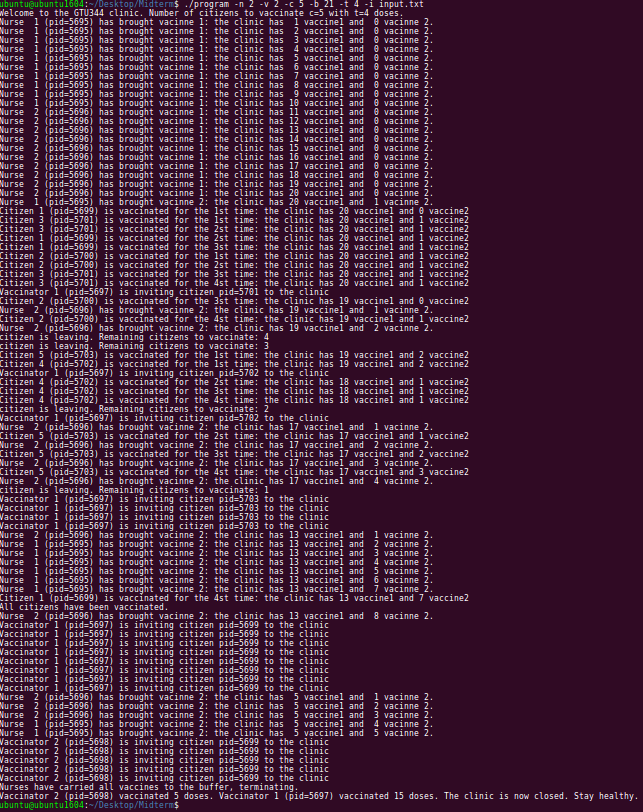
\includegraphics[width=1\textwidth, left]{output.png}
\caption[Optional caption]{}
\label{}
\end{figure}                    
\end{document}